\lab{Algorithms}{Interior Point I}{Interior Point I}
\objective{Learn About Interior Point Methods for Linear Programming}

\section*{Interior Point Methods: Overview}
Although the Simplex Algorithm was long the only practically competitive method for linear programming, the past 30 years has seen the discovery and widespread adoption of a new family of algorithms that rival and in some cases outperform the Simplex Algorithm, collectively called Interior Point methods. One of the major shortcomings of the Simplex Algorithm is that the number of steps required to solve the problem can grow exponentially in the size of the linear system. Thus, for certain large linear programs, the Simplex Algorithm is simply not viable. In practice, however, such pathological examples are rarely encountered. Interior Point methods offer and alternative approach and guarantee much better theoretical convergence properties.

Recall that a linear program is a constrained optimization problem with a linear objective function and linear constraints.
The linear constraints define a set of allowable points called the \emph{feasible region}, the boundary of which forms a geometric
object known as a \emph{polytope}. The theory of convex optimization ensures that the optimal point for the objective function
can be found among the vertices of the feasible polytope. The Simplex Method tests a sequence of such vertices until it finds
the optimal point. Provided the linear program is neither unbounded nor infeasible, the algorithm is certain to produce the correct
answer after a finite number of steps, but it does not guarantee an efficient path along the polytope toward the minimizer. Interior point methods do away with the feasible polytope and instead generate a sequence of points that cut through the interior (or
exterior) of the feasible region and converge iteratively to the optimal point. Although it is computationally more expensive to
compute such interior points, each step results in significant progress toward the minimizer. See Figure \ref{intPoint:intPath} for
a visualization of an Interior Point method. In general, the Simplex Method requires many more, albeit less expensive, computations.

\begin{figure}
\centering
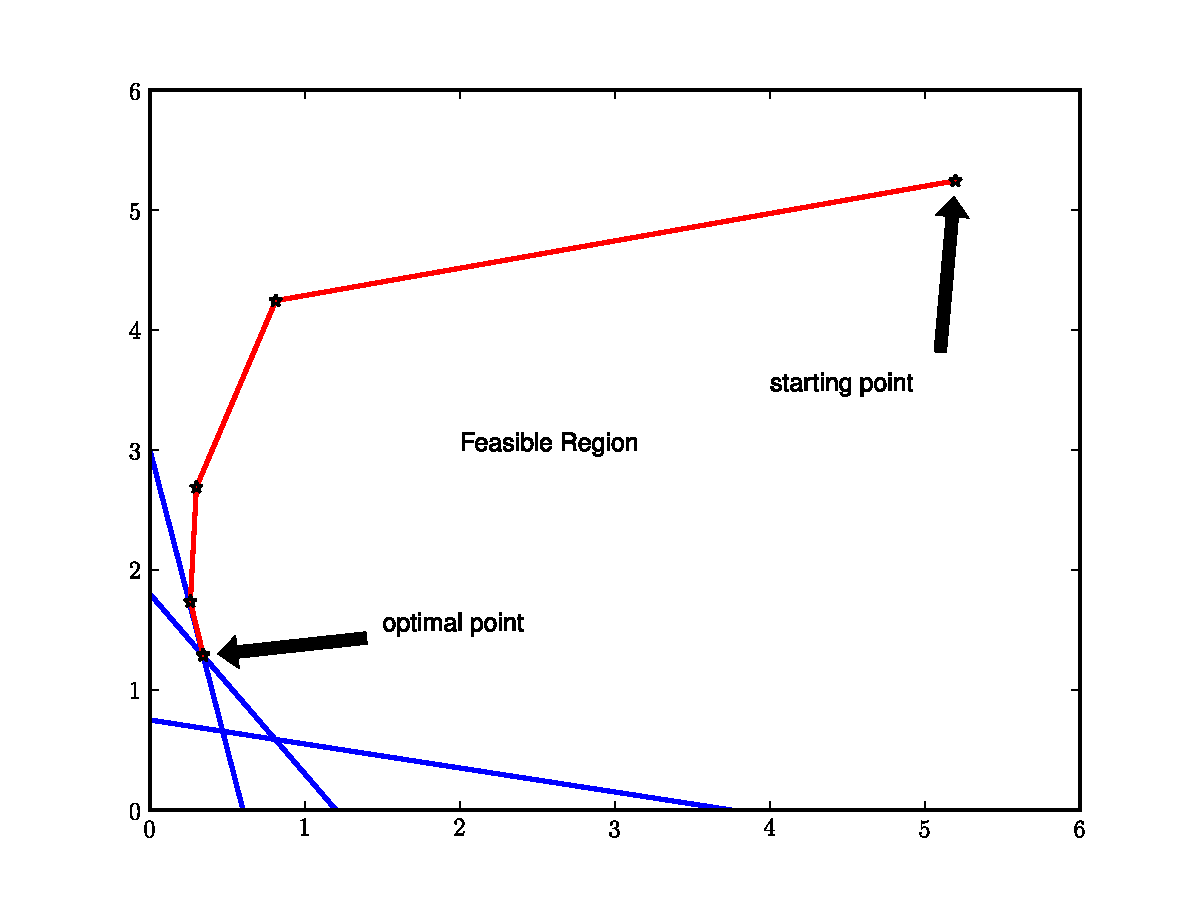
\includegraphics[width=\textwidth]{interiorPath.pdf}
\caption{A path traced by an Interior Point algorithm.}
\label{intPoint:intPath}
\end{figure}

\section*{Primal-Dual Interior Point Methods}
The most popular and successful types of Interior Point methods nowadays are known as Primal-Dual Interior Point methods. To
describe this approach, let us consider the following linear program:
\begin{align*}
\text{minimize } &c^Tx\\
\text{subject to } &Ax = b\\
&x \geq 0.
\end{align*}
Here, $x, c \in \mathbb{R}^n$, $b \in \mathbb{R}^m$, and $A$ is an $m \times n$ matrix with full row rank. By $x \geq 0$, we
simply mean that each coordinate of $x$ is nonnegative. Note that this formulation is quite general, as any linear program can be
posed in this manner, after appropriate transformations. This is the primal problem, and its dual takes the form
\begin{align*}
\text{maximize } &b^T\lambda\\
\text{subject to } &A^T\lambda + s = c\\
&s \geq 0,
\end{align*}
where $\lambda \in \mathbb{R}^m$ and $s \in \mathbb{R}^n$. The theory of convex optimization gives us necessary and sufficient
conditions for the solutions to the primal and dual problems via the Karush-Kuhn-Tucker conditions, which in this case take the form
\begin{align*}
A^T\lambda + s &= c\\
Ax &= b\\
x_is_i &= 0, \,\,\, i = 1,2,\ldots,n\\
x, s &\geq 0.
\end{align*}
A Primal-Dual Interior Point method is a line search method that starts with an initial guess $(x_0, \lambda_0, s_0)$
and produces a sequence of points that converge to $(x^*, \lambda^*, s^*)$, the solution to the KKT equations and hence
the solution to the original linear program.

\subsection*{Search Direction and Step Length}
We now describe how to select the search direction and step length at each iteration of the algorithm. Because this is 
a constrained problem, matters are more complicated than is usual in unconstrained line search methods.

The top three lines of the KKT conditions can be re-written as one large almost-linear homogeneous system of equations. 
In the spirit of
Newton's Method, we can form a linear approximation of this system centered around our current point $(x, \lambda, s)$, and
calculate the direction $(\triangle x, \triangle \lambda, \triangle s)$ in which to step in order to set the linear approximation
equal to 0. This equates to solving the linear system
\begin{equation}
\begin{bmatrix}
0 & A^T & I\\
A & 0 & 0\\
S & 0 & X
\end{bmatrix}
\begin{bmatrix}
\triangle x\\
\triangle \lambda\\
\triangle s
\end{bmatrix}
=
\begin{bmatrix}
-r_c\\
-r_b\\
-XSe
\end{bmatrix},
\label{eq:affine}
\end{equation}
where $r_b = Ax - b,$ $r_c = A^T\lambda + s - c$, $I$ is an appropriately-sized identity matrix, $X = \text{diag}(x_1,\ldots,x_n),$
$S = \text{diag}(s_1,\ldots,s_n)$, and $e = (1,1,\ldots,1)^T$.
This Newton direction is too greedy, however, and even small steps in this direction may cause us to violate the nonnegativity
condition (the last line of the KKT conditions). We need to find a new search direction.

Choosing an appropriate search direction is a tricky task, and various approaches exist. We will follow a popular strategy 
known as the \emph{Predictor-Corrector Algorithm}. The idea is to actually calculate two directions. We first calculate 
the standard Newton direction described above; that is, we obtain the solution to Equation \ref{eq:affine}. This is known as
the \emph{predictor step}, since it gives us a direction in which the objective does indeed decrease, hence predicting our
final search direction. Denote the solution to this system by $(\triangle x^a, \triangle \lambda^a, \triangle s^a)$.
As discussed, however, we must deviate from this direction somewhat, and so we additionally solve the
following linear system of equations:
\begin{equation}
\begin{bmatrix}
0 & A^T & I\\
A & 0 & 0\\
S & 0 & X
\end{bmatrix}
\begin{bmatrix}
\triangle x\\
\triangle \lambda\\
\triangle s
\end{bmatrix}
=
\begin{bmatrix}
-r_c\\
-r_b\\
-XSe - \triangle X^a\triangle S^ae + \sigma \mu e
\end{bmatrix}.
\label{eq:centering}
\end{equation}
The solution to this system, which we denote by $(\triangle x, \triangle \lambda, \triangle s)$, is our final search direction.
Note that $\triangle X^a = \text{diag}(\triangle x_1^a,\ldots,\triangle x_n^a)$, $\triangle S^a = \text{diag}(\triangle s_1^a,\ldots,\triangle s_n^a)$. Further, define $\mu := x^Ts/n$. The formula for $\sigma$ is somewhat more complicated, and
is based on a heuristic approach. Make the following calculations:
\begin{align*}
\alpha_a^p &:= \min\left(1, \displaystyle\min_{i : \triangle x_i^a < 0}-\frac{x_i}{\triangle x_i^a}\right)\\
\alpha_a^d &:= \min\left(1, \displaystyle\min_{i : \triangle s_i^a < 0}-\frac{s_i}{\triangle s_i^a}\right).
\end{align*}
Next, define
$$
\mu_a := (x+\alpha_a^p\triangle x^a)^T(s+\alpha_a^d\triangle s^a)/n.
$$
Finally, calculate $\sigma$ by the formula
$$
\sigma = \left(\frac{\mu_a}{\mu}\right)^3.
$$

Now that we have our search direction, it remains to choose our step length. We wish to step nearly as far as possible without
violating the nonnegativity condition, thus remaining in the interior of the feasible region. First, make the following
calculations:
\begin{align*}
\beta^p &:= \displaystyle\min_{i : \triangle x_i < 0}-\frac{x_i}{\triangle x_i}\\
\beta^d &:= \displaystyle\min_{i : \triangle s_i < 0}-\frac{s_i}{\triangle s_i}.
\end{align*}
Next, calculate
\begin{align*}
\alpha^p &:= \min(1, 0.95\beta^p)\\
\alpha^d &:= \min(1, 0.95\beta^d).
\end{align*}
These are our step lengths. That is, our next point $(x', \lambda', s')$ is given by
\begin{align*}
x' &= x + \alpha^p\triangle x\\
(\lambda', s') &= (\lambda, s) + \alpha^d(\triangle \lambda, \triangle s).
\end{align*}
We summarize the entire procedure in Algorithm \ref{alg:predcorr}.
\begin{algorithm}
\begin{algorithmic}[1]
\Procedure{Predictor-Corrector Algorithm}{}
    \State \textrm{Choose initial point } $(x_0, \lambda_0, s_0)$.
    \For{$k = 0, 1, 2, \ldots$}
        \State \textrm{Solve for } $(\triangle x^a, \triangle \lambda^a, \triangle s^a)$.
        \State \textrm{Calculate } $\alpha_a^p, \alpha_a^d, \mu_a$, \textrm{and} $\sigma$.
        \State \textrm{Solve for } $(\triangle x, \triangle \lambda, \triangle s)$.
        \State \textrm{Calculate the step lengths } $\alpha^p, \alpha^d$.
        \State \textrm{Step to the new point: } $x_{k+1} = x_k + \alpha^p\triangle x$, 
        $(\lambda_{k+1}, s_{k+1}) = (\lambda_k, s_k) + \alpha^d(\triangle \lambda, \triangle s)$.
    \EndFor
\EndProcedure
\end{algorithmic}
\caption{Predictor-Corrector Algorithm}
\label{alg:predcorr}
\end{algorithm}
